\documentclass[preprint,12pt]{elsarticle}
\biboptions{numbers,sort&compress}

\usepackage{amsmath,amssymb,amsfonts}
\usepackage{graphicx}
\usepackage{booktabs}

\usepackage{url}
\usepackage{hyperref}



\usepackage{microtype}
\usepackage{tabularx}
\usepackage{lineno}



\journal{Sustainable Computing: Informatics and Systems}


\providecommand{\tightlist}{\setlength{\itemsep}{0pt}\setlength{\parskip}{0pt}}
\providecommand{\real}[1]{#1}
\begin{document}

\begin{frontmatter}

\title{SHIFT-GPU: Shift-Aware, Risk-Calibrated and Physics-Guided Learning for Reliable LLM Inference Hardware Selection}

\author[inst1]{Jason Pandian\corref{cor1}}
\ead{pandiajason@gmail.com}

\cortext[cor1]{Corresponding author. Department of Information Technology, Nehru Institute of Technology, Coimbatore, Tamil Nadu, 641105, India.}

\affiliation[inst1]{organization={Department of Information Technology, Nehru Institute of Technology},
            addressline={Thirumalayampalayam}, 
            city={Coimbatore},
            postcode={641105}, 
            state={Tamil Nadu}, 
            country={India}}

\begin{abstract}
Selecting GPUs for large language model (LLM) serving requires balancing
inference latency and operating power when measurements on the target
hardware are scarce. SHIFT-GPU combines a Roofline-based latency prior,
workload-conditioned attention over GPU features, empirical adjustment
of latency intervals, and budgeted profiling. We evaluate the framework
through leave-one-GPU-out prediction and offline selection on 4,163
benchmark executions across eight NVIDIA GPU models. We compare GPU
selection policies at a 35 ms mean inter-token latency threshold and
distinguish prediction coverage from the observed failure rate of
selected configurations. SHIFT-GPU achieved 15.87\% latency MdAPE
compared with 11.28\% for matched XGBoost. Distance inflation increased
empirical coverage from 88.30\% to 94.02\%. In offline replay, both
policies admitted all 125 workloads. Using the upper latency bound
reduced observed violations from one to zero while increasing mean
selected power from 124.06 W to 145.74 W. The study measures power and
uses archived profiling observations. Energy savings and production
performance require separate validation.
\end{abstract}
\begin{highlights}

\item
  A workload query attends to distinct hardware feature tokens.
\item
  Eight leave-one-GPU-out folds test transfer to held-out GPU models.
\item
  Interval widening raises empirical coverage from 88.30\% to 94.02\%.
\item
  Offline replay measures the power cost of reducing latency violations.
\end{highlights}
\begin{keyword}
Large Language Models \sep GPU Infrastructure \sep Physics-Informed Neural Networks \sep Conformal Prediction \sep Active Learning \sep Sustainable Computing.
\end{keyword}

\end{frontmatter}

\linenumbers
\emergencystretch=2em

\section{Introduction}\label{introduction}

Large language model (LLM) serving places substantial computational
demands on cloud infrastructure. Infrastructure operators select
accelerators that meet response-time targets while controlling GPU
power. This paper evaluates one such target, mean inter-token latency
(ITL), for hardware with no training measurements.

To optimize throughput per Watt, modern cloud providers deploy
heterogeneous GPU clusters spanning multiple architectural generations,
including NVIDIA Hopper (H100, H200), Ada Lovelace (L40S, L4), Ampere
(A100, A30), Turing (T4), and Volta (V100). When an infrastructure
operator seeks to deploy a new LLM workload, they must decide:
\emph{Which GPU candidate satisfies the required latency SLA with the
lowest operational power draw?}

Traditionally, answering this question requires exhaustive physical
profiling: systematically deploying the LLM across every candidate
accelerator under varying prompt lengths, concurrency arrival rates, and
batch sizes. However, with dozens of active foundation models and
hundreds of potential accelerator configurations, empirical profiling
incurs massive energy consumption, creates severe scheduling overhead,
and delays workload onboarding.

\subsection{Research Contributions}\label{research-contributions}

\begin{enumerate}
\def\labelenumi{\arabic{enumi}.}
\tightlist
\item
  A Roofline-guided predictor with workload-conditioned attention across
  hardware features.
\item
  An empirical evaluation of latency interval adjustment and power-aware
  selection under a latency service-level agreement.
\item
  A comparison of four limited-profiling strategies on a shared held-out
  evaluation subset.
\end{enumerate}

\section{Related Work}\label{related-work}

Castaño et al.~{[}1{]} use MLPerf measurements to predict throughput and
energy per unit and recommend hardware along a performance, energy, and
cost frontier. Aguirre-Usandizaga et al.~{[}2{]} forecast GPU power from
high-frequency telemetry for proactive load allocation in LLM serving.
These studies motivate two different decisions: selecting hardware
across measured configurations and allocating workloads on an observed
cluster. Our question is whether predictive latency intervals and a few
targeted measurements can improve deployment choices when an individual
GPU model is held out.

WattGPU {[}3{]} is the closest baseline for predicting inference power
and inter-token latency (ITL) from public model and GPU metadata. Its
benchmark and leave-one-GPU-out protocol provide the starting point for
this work. IBM's Roofline-driven ML study {[}4{]} and NeuSight {[}5{]}
establish prior art for physically informed inference prediction and
performance transfer to unseen GPUs. The proposed contribution is the
combined evaluation of latency-aware hardware selection and budgeted
profiling in this setting. Weighted conformal inference under covariate
shift {[}6{]} uses assumptions about the conditional response
distribution and density ratios. Our distance adjustment is evaluated
empirically and has no corresponding coverage theorem.

\section{Problem Formulation}
\label{sec:formulation}

\subsection{Inference Workload and Hardware Specification Spaces}
Let an LLM inference workload be defined as a tuple $x = (m, s) \in \mathcal{X}$, where $m \in \mathcal{M}$ represents the model architecture metadata and $s \in \mathcal{S}$ represents the operational serving scenario. Specifically, $m$ includes parameter count $N_{\text{params}}$, hidden dimension $H$, layer count $L$, attention head count $N_h$, key-value head count $N_{kv}$, and KV-cache footprint $C_{kv}$. The operational scenario $s \in \{\text{offline}, \text{server\_low}, \text{server\_high}\}$ specifies the request arrival process and batching dynamics.

Let a candidate hardware accelerator be defined as a vector $g \in \mathcal{G}$, characterized by microarchitectural parameters: memory bandwidth $B_{\text{mem}}$ (GB/s), peak FP16 compute capacity $F_{\text{peak}}$ (TFLOPS), device memory capacity $M_{\text{size}}$ (GB), Thermal Design Power $TDP$ (Watts), base clock frequency $f_{\text{base}}$ (MHz), boost ratio $\kappa_{\text{boost}}$, transistor count $C_{\text{trans}}$, and architectural family generation $A_{\text{gen}} \in \{\text{Volta}, \text{Turing}, \text{Ampere}, \text{Ada}, \text{Hopper}\}$.

For any workload-hardware pair $(x, g)$, the system exhibits two ground-truth execution properties:
\begin{enumerate}
    \item Inter-Token Latency (ITL): $T(x, g) \in \mathbb{R}^+$ (seconds per token).
    \item Mean Operational Power Draw: $P(x, g) \in \mathbb{R}^+$ (Watts).
\end{enumerate}

\subsection{The Constrained Hardware Selection Problem}
Given a target workload $x \in \mathcal{X}$ and a latency Service Level Agreement threshold $T_{\max} \in \mathbb{R}^+$, the cluster scheduler's objective is to select the accelerator $g^* \in \mathcal{G}$ that minimizes operational power consumption while satisfying the latency constraint using an empirical upper latency estimate:
\begin{equation}
\label{eq:opt_problem}
g^* = \arg\min_{g \in \mathcal{G}} \hat P(x, g) \quad \text{subject to} \quad U(x,g) \le T_{\max}
\end{equation}

When ground truth measurements $T(x, g)$ and $P(x, g)$ are unavailable, the selection must rely on surrogate predictors $\hat{T}(x, g)$ and $\hat{P}(x, g)$. If a model relies purely on point estimates $\hat{T}(x, g) \le T_{\max}$, any prediction underestimation ($\hat{T} \le T_{\max} < T$) results in an operational SLA violation. 

\subsection{Operational Regret Formulation}
To rigorously quantify the cost of suboptimal hardware selection, we formalize the operational deployment regret $\mathcal{R}(g^* \mid x)$ relative to the true empirical Oracle accelerator $g_{\text{oracle}}$:
\begin{equation}
\label{eq:regret}
\begin{aligned}\mathcal{R}(g^* \mid x) ={}& \max\left(0, P(x, g^*) - P(x, g_{\text{oracle}})\right) \\ &+ \lambda_{\text{SLA}} \cdot P(x, g^*) \cdot \mathbb{I}\left(T(x, g^*) > T_{\max}\right)
\end{aligned}
\end{equation}
where $\mathbb{I}(\cdot)$ is the indicator function and $\lambda_{\text{SLA}} \ge 1$ is an asymmetric penalty factor reflecting the commercial penalty of SLA breach.

\section{The SHIFT-GPU Methodology}\label{the-shift-gpu-methodology}

\subsection{Physics-guided
prediction}\label{physics-guided-prediction}

The Roofline model {[}7{]} motivates a latency prior defined as the
maximum of estimated FP16 weight-streaming time and peak compute time.
The weight-streaming term divides by an assumed batching factor of 256
offline and 1 in server mode. These are scenario-level assumptions. The
power head scales a sigmoid prediction by GPU thermal design power
(TDP). The resulting floor and cap constrain model outputs. Their
accuracy depends on the operating conditions and GPU specifications.

The workload encoder produces a query. The hardware encoder supplies one
summary token. Each normalized continuous hardware feature supplies a
separate token through a shared scalar projection plus a learned feature
identity. The workload query attends to all hardware tokens using four
heads. This allows attention weights to vary with the workload. The ITL
head multiplies the prior by one plus the exponential of its learned
residual. The model learns heteroscedastic uncertainty in log-latency
for ITL and in TDP-normalized units for power. For ITL, we approximate
the standard deviation in seconds by multiplying the log-scale standard
deviation by predicted latency.

\subsection{Calibration on source
hardware}\label{calibration-on-source-hardware}

For each held-out GPU, we reserve 20\% of the source rows for
calibration. Numerical scaling and category vocabularies are fit on the
remaining training rows, with unknown categories assigned to a fixed
zero embedding. The model trains for 35 epochs using AdamW at a learning
rate of 0.0015, batch size 64, and seed 42. We compute absolute
standardized calibration residuals and use rank ceiling((n + 1) × 0.90)
to obtain the quantile. The adjusted interval multiplies this quantile
by 1 + 0.15 × min(d, 5), where d is the regularized Mahalanobis distance
from the training GPUs, each counted once. The multiplier saturates at
1.75. We report two-sided row-level coverage and separately evaluate
violations among admitted workloads. Neither statistic implies a
guarantee for future hardware or for the chosen candidate.

\subsection{Budgeted profiling}\label{budgeted-profiling}

We set aside 20\% of each target GPU's benchmark rows as possible probes
and evaluate every strategy on the same remaining rows. The strategies
select up to one, three, or five probes using random sampling, workload
diversity, predicted uncertainty, or an SLA boundary heuristic. The
heuristic combines predicted ITL standard deviation, Gaussian proximity
to 35 ms, and normalized predicted power. Profiling updates the latency
prediction by a shrunk median ratio of measured to predicted ITL. The
few-shot experiment evaluates prediction error separately from the
hardware replay, which uses zero-shot predictions.


\paragraph{Prediction heads and acquisition score.}
Let $H_g$ denote the matrix containing the hardware summary token and the eight continuous feature tokens.
The attention block uses $Q=W_q w_x$, $K=H_gW_k$, and $V=H_gW_v$. The latency and power heads use
\[
\hat T=T_{\rm roof}(1+\exp r_\theta),\qquad
\hat P=\mathrm{TDP}\cdot\operatorname{sigmoid}(p_\theta).
\]
The SLA boundary acquisition score used in the experiments is
\[
\begin{aligned}a(x)={}&\sigma(x)\left[0.1+\exp\left(-\frac{1}{2}
\left(\frac{\hat T(x)-T_{\max}}{\sigma(x)+10^{-6}}\right)^2\right)\right]\\
&\quad \left[0.1+\frac{\hat P(x)}{\max_{x'\,\in\,\mathcal P_g}\hat P(x')+10^{-6}}\right],
\end{aligned}
\]
where $\mathcal P_g$ is the profiling pool for GPU $g$.
\section{Experimental Setup}\label{experimental-setup}

The benchmark contains eight GPU models across five architecture
families. Each of the eight outer folds holds out one GPU model
completely during training and calibration. This tests transfer to an
unseen model and may leave a related GPU from the same family available
for training. We report pooled median absolute percentage error (MdAPE),
empirical interval coverage, and per-device errors. In offline hardware
replay, repeated records for each model, serving scenario, and GPU are
summarized by their medians. We report violations among admitted
workloads, abstention among all workloads, and mean power of selected
GPUs. The retrospective oracle uses observed median values. Regret adds
5 times observed power for a violation and assigns a fixed penalty of
100 to abstention when a feasible GPU exists.

\subsection{Hardware Accelerator Population}
The evaluated accelerators span five distinct NVIDIA architectural generations, summarized in Table \ref{tab:hardware_specs}.

\begin{table}[h]
\centering
\caption{Microarchitectural specifications of evaluated server-grade GPU hardware population.}
\label{tab:hardware_specs}
\resizebox{\linewidth}{!}{%
\begin{tabular}{llrrrrrr}
\toprule
\textbf{GPU Model} & \textbf{Architecture} & \textbf{Release} & \textbf{Mem (GB)} & \textbf{BW (GB/s)} & \textbf{TFLOPS} & \textbf{TDP (W)} & \textbf{Process} \\
\midrule
Tesla V100 SXM2 & Volta & 2018 & 32.0 & 898.0 & 125.0 & 300 & 12 nm \\
Tesla T4 & Turing & 2018 & 16.0 & 320.0 & 65.0 & 70 & 12 nm \\
A100 SXM4 & Ampere & 2020 & 40.0 & 1560.0 & 312.0 & 400 & 7 nm \\
A30 PCIe & Ampere & 2021 & 24.0 & 933.1 & 165.0 & 165 & 7 nm \\
L40S & Ada Lovelace & 2022 & 48.0 & 864.0 & 362.0 & 350 & 5 nm \\
L4 & Ada Lovelace & 2023 & 24.0 & 300.1 & 121.0 & 72 & 5 nm \\
H100 NVL & Hopper & 2023 & 94.0 & 3940.0 & 835.0 & 400 & 5 nm \\
H200 NVL & Hopper & 2024 & 141.0 & 4890.0 & 835.0 & 700 & 5 nm \\
\bottomrule
\end{tabular}%
}
\end{table}

\section{Experimental Results and
Analysis}\label{experimental-results-and-analysis}

\subsection{Held-out GPU prediction}\label{held-out-gpu-prediction}

The matched XGBoost reference uses WattGPU-style features and
hyperparameters on the same source training rows and held-out GPUs.
SHIFT-GPU achieved \textbf{15.87\% ITL MdAPE} and \textbf{21.98\% power
MdAPE}. The matched gradient-boosted reference achieved \textbf{11.28\%}
and \textbf{12.35\%}, respectively. The raw Roofline and TDP references
gave \textbf{38.10\%} and \textbf{104.09\%} error. The study does not
establish a predictive improvement over the matched tree baseline.

\begin{table}[htbp]
\centering
\caption{Held-out GPU prediction errors}
\resizebox{0.95\linewidth}{!}{\begin{tabular}{lrr}
\toprule
Held-out GPU & ITL MdAPE (\%) & Power MdAPE (\%) \\
\midrule
A30 PCIe & 74.24 & 19.64 \\
H200 NVL & 10.16 & 24.14 \\
A100 SXM4 40 GB & 11.13 & 44.06 \\
L40S & 15.19 & 12.98 \\
H100 NVL 94 GB & 8.02 & 22.86 \\
Tesla V100 SXM2 32 GB & 29.22 & 46.20 \\
L4 & 16.61 & 26.54 \\
Tesla T4 & 10.83 & 14.87 \\
\end{tabular}}
\end{table}

\begin{figure}
\centering
{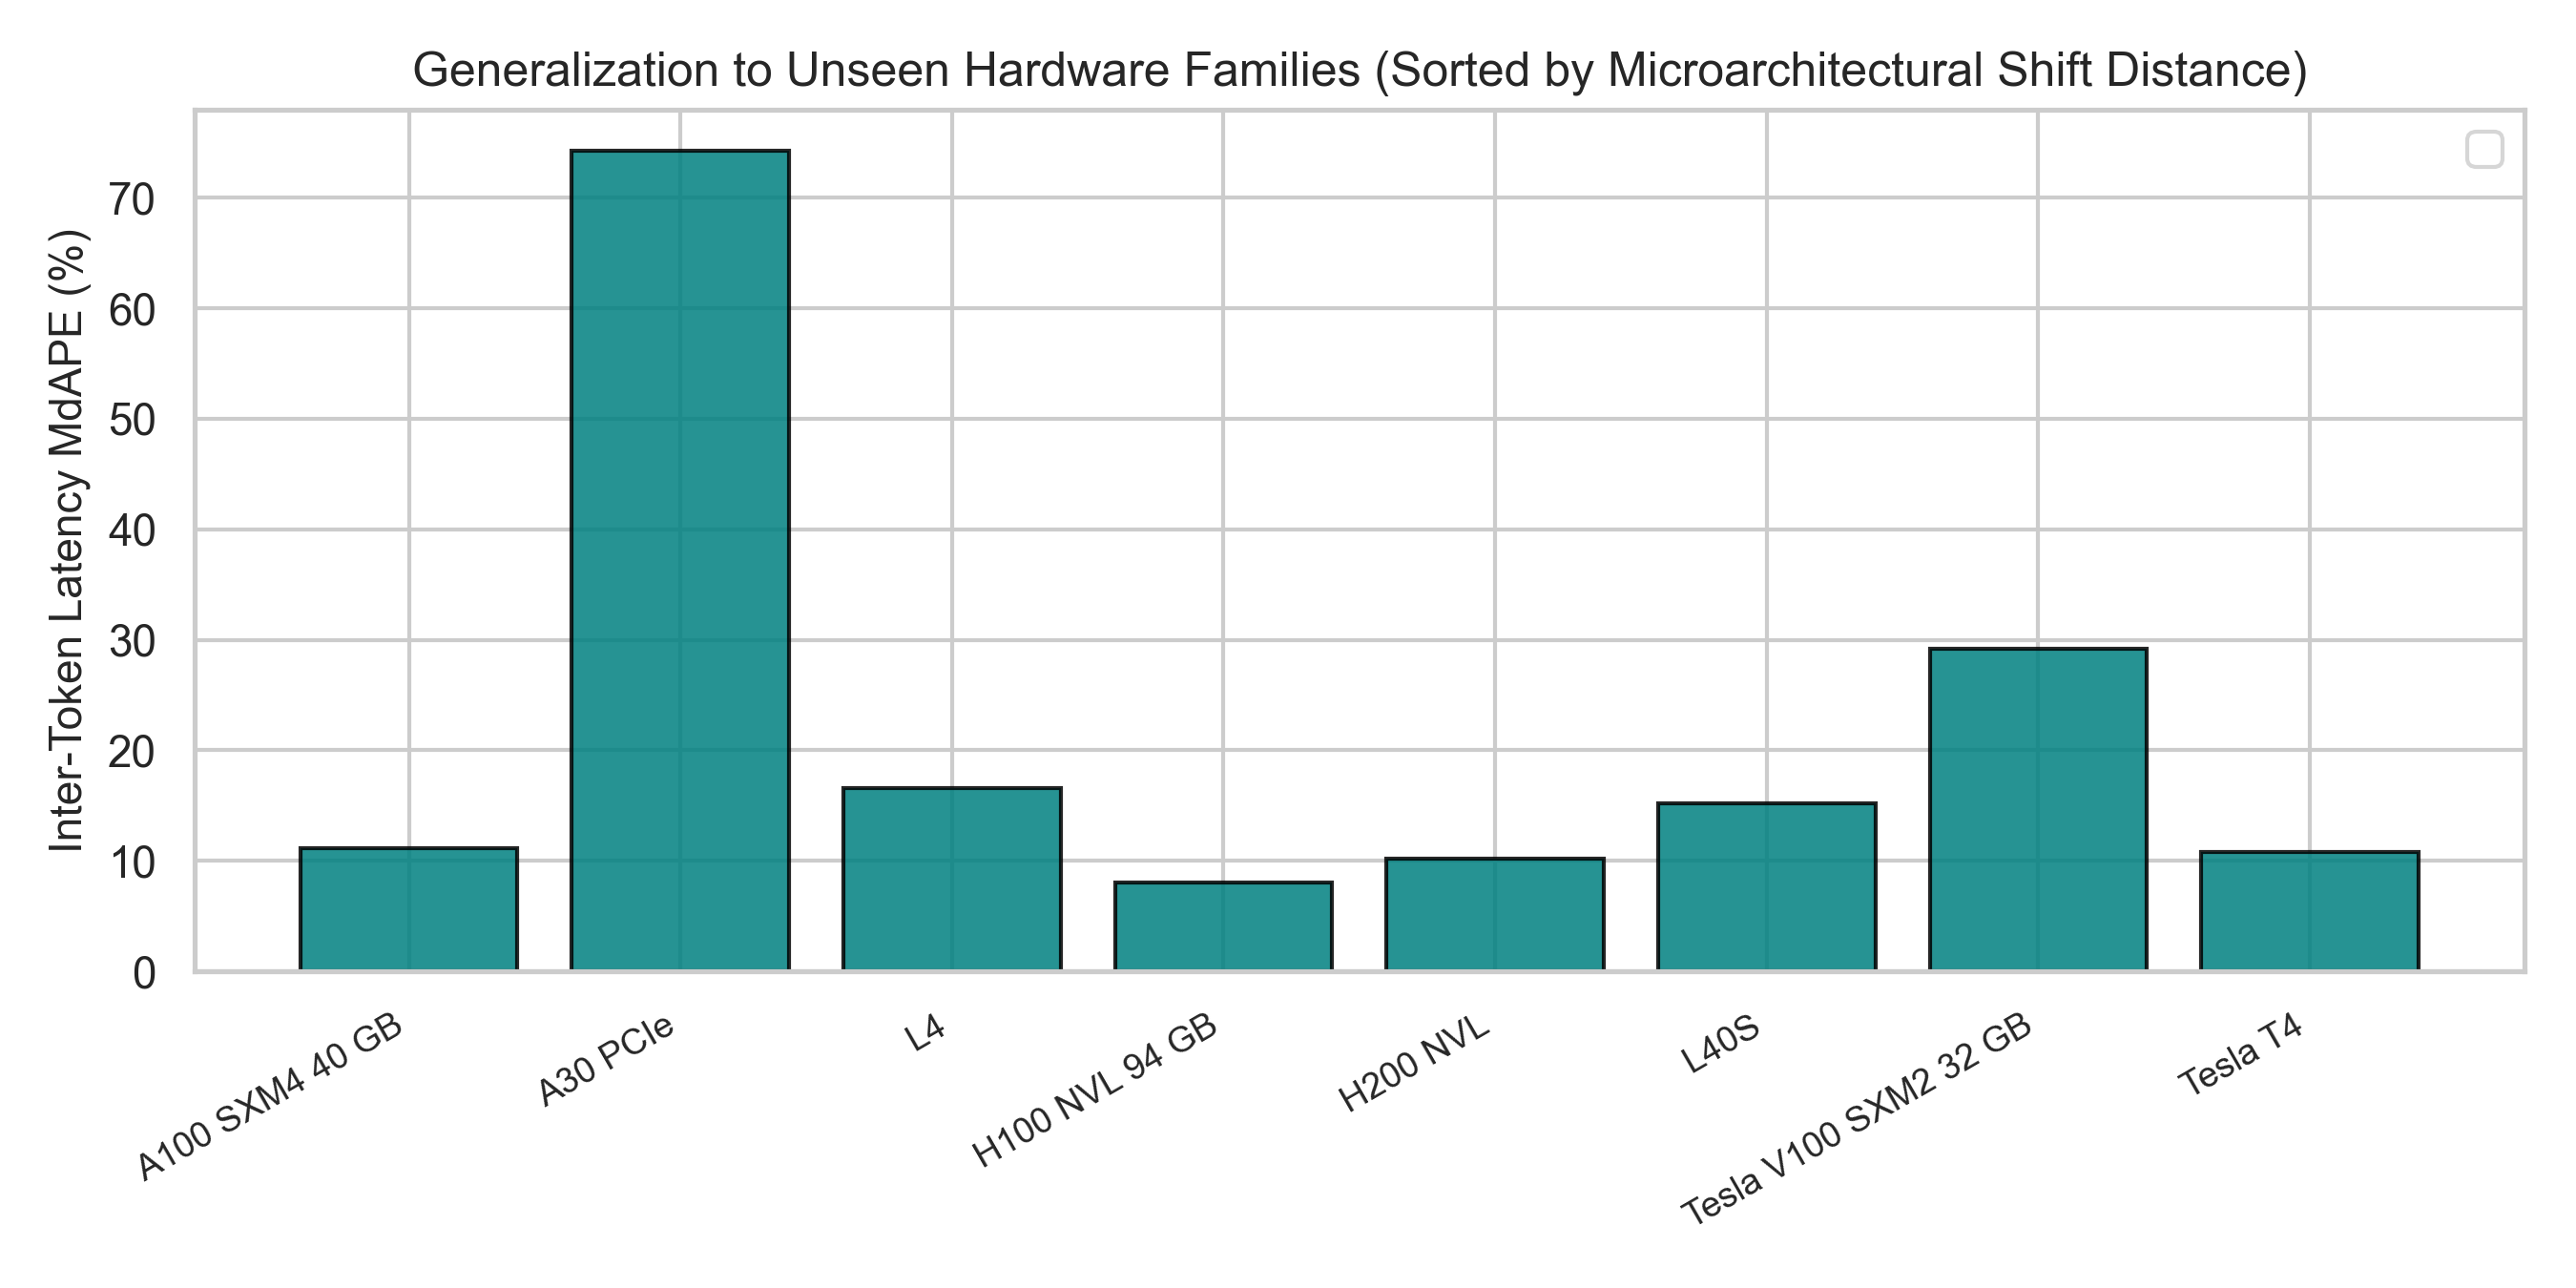
\includegraphics[width=0.84\linewidth]{figures/fig1_unseen_hardware_generalization.png}}
\caption{Zero-shot latency error by GPU, ordered by hardware
distance.}
\end{figure}

\subsection{Latency uncertainty and offline hardware
selection}\label{latency-uncertainty-and-offline-hardware-selection}

Two-sided empirical coverage was \textbf{88.30\%} without the distance
multiplier and \textbf{94.02\%} with it, against a nominal target of
90\%. All eight distances exceeded the cap, so the adjusted method was
equivalent to a single global inflation factor on this dataset. The
replay evaluates policies at the same 35 ms threshold. Both learned
policies admitted 125 workloads. The interval policy avoided one
observed violation while increasing average selected power by 21.69 W
and raising mean regret under the specified penalty. This result
illustrates a trade-off between latency risk and power.

\begin{table}[htbp]
\centering
\caption{Offline recommendation under the 35 ms latency threshold}
\resizebox{0.95\linewidth}{!}{\begin{tabular}{lrrrrr}
\toprule

Selection policy
 & 
Admitted
 & 
Violation (\% admitted)
 & 
Abstained (\%)
 & 
Selected power (W)
 & 
Mean regret
 \\
\midrule
Point Estimate & 125/125 & 0.80 & 0.00 & 124.06 & 14.52 \\
Risk Calibrated & 125/125 & 0.00 & 0.00 & 145.74 & 33.58 \\
Min Tdp & 125/125 & 0.80 & 0.00 & 116.62 & 7.09 \\
Oracle & 125/125 & 0.00 & 0.00 & 112.16 & 0.00 \\
\end{tabular}}
\end{table}

\subsection{Budgeted profiling}\label{budgeted-profiling-1}

\begin{table}[htbp]
\centering
\caption{Few-shot latency prediction results}
\resizebox{0.95\linewidth}{!}{\begin{tabular}{rlr}
\toprule
Probe budget & Selection strategy & ITL MdAPE (\%) \\
\midrule
0 & No adaptation & 15.84 \\
1 & Random & 13.18 \\
1 & Diversity & 13.87 \\
1 & Uncertainty & 17.20 \\
1 & Sla Boundary & 19.21 \\
3 & Random & 9.30 \\
3 & Diversity & 9.38 \\
3 & Uncertainty & 9.86 \\
3 & Sla Boundary & 18.90 \\
5 & Random & 9.61 \\
5 & Diversity & 9.64 \\
5 & Uncertainty & 11.07 \\
5 & Sla Boundary & 18.52 \\
\end{tabular}}
\end{table}

The lowest error was \textbf{9.30\%} using random at budget 3. Results
are from one fixed split and do not establish that an acquisition rule
minimizes deployment regret.

\begin{figure}
\centering
{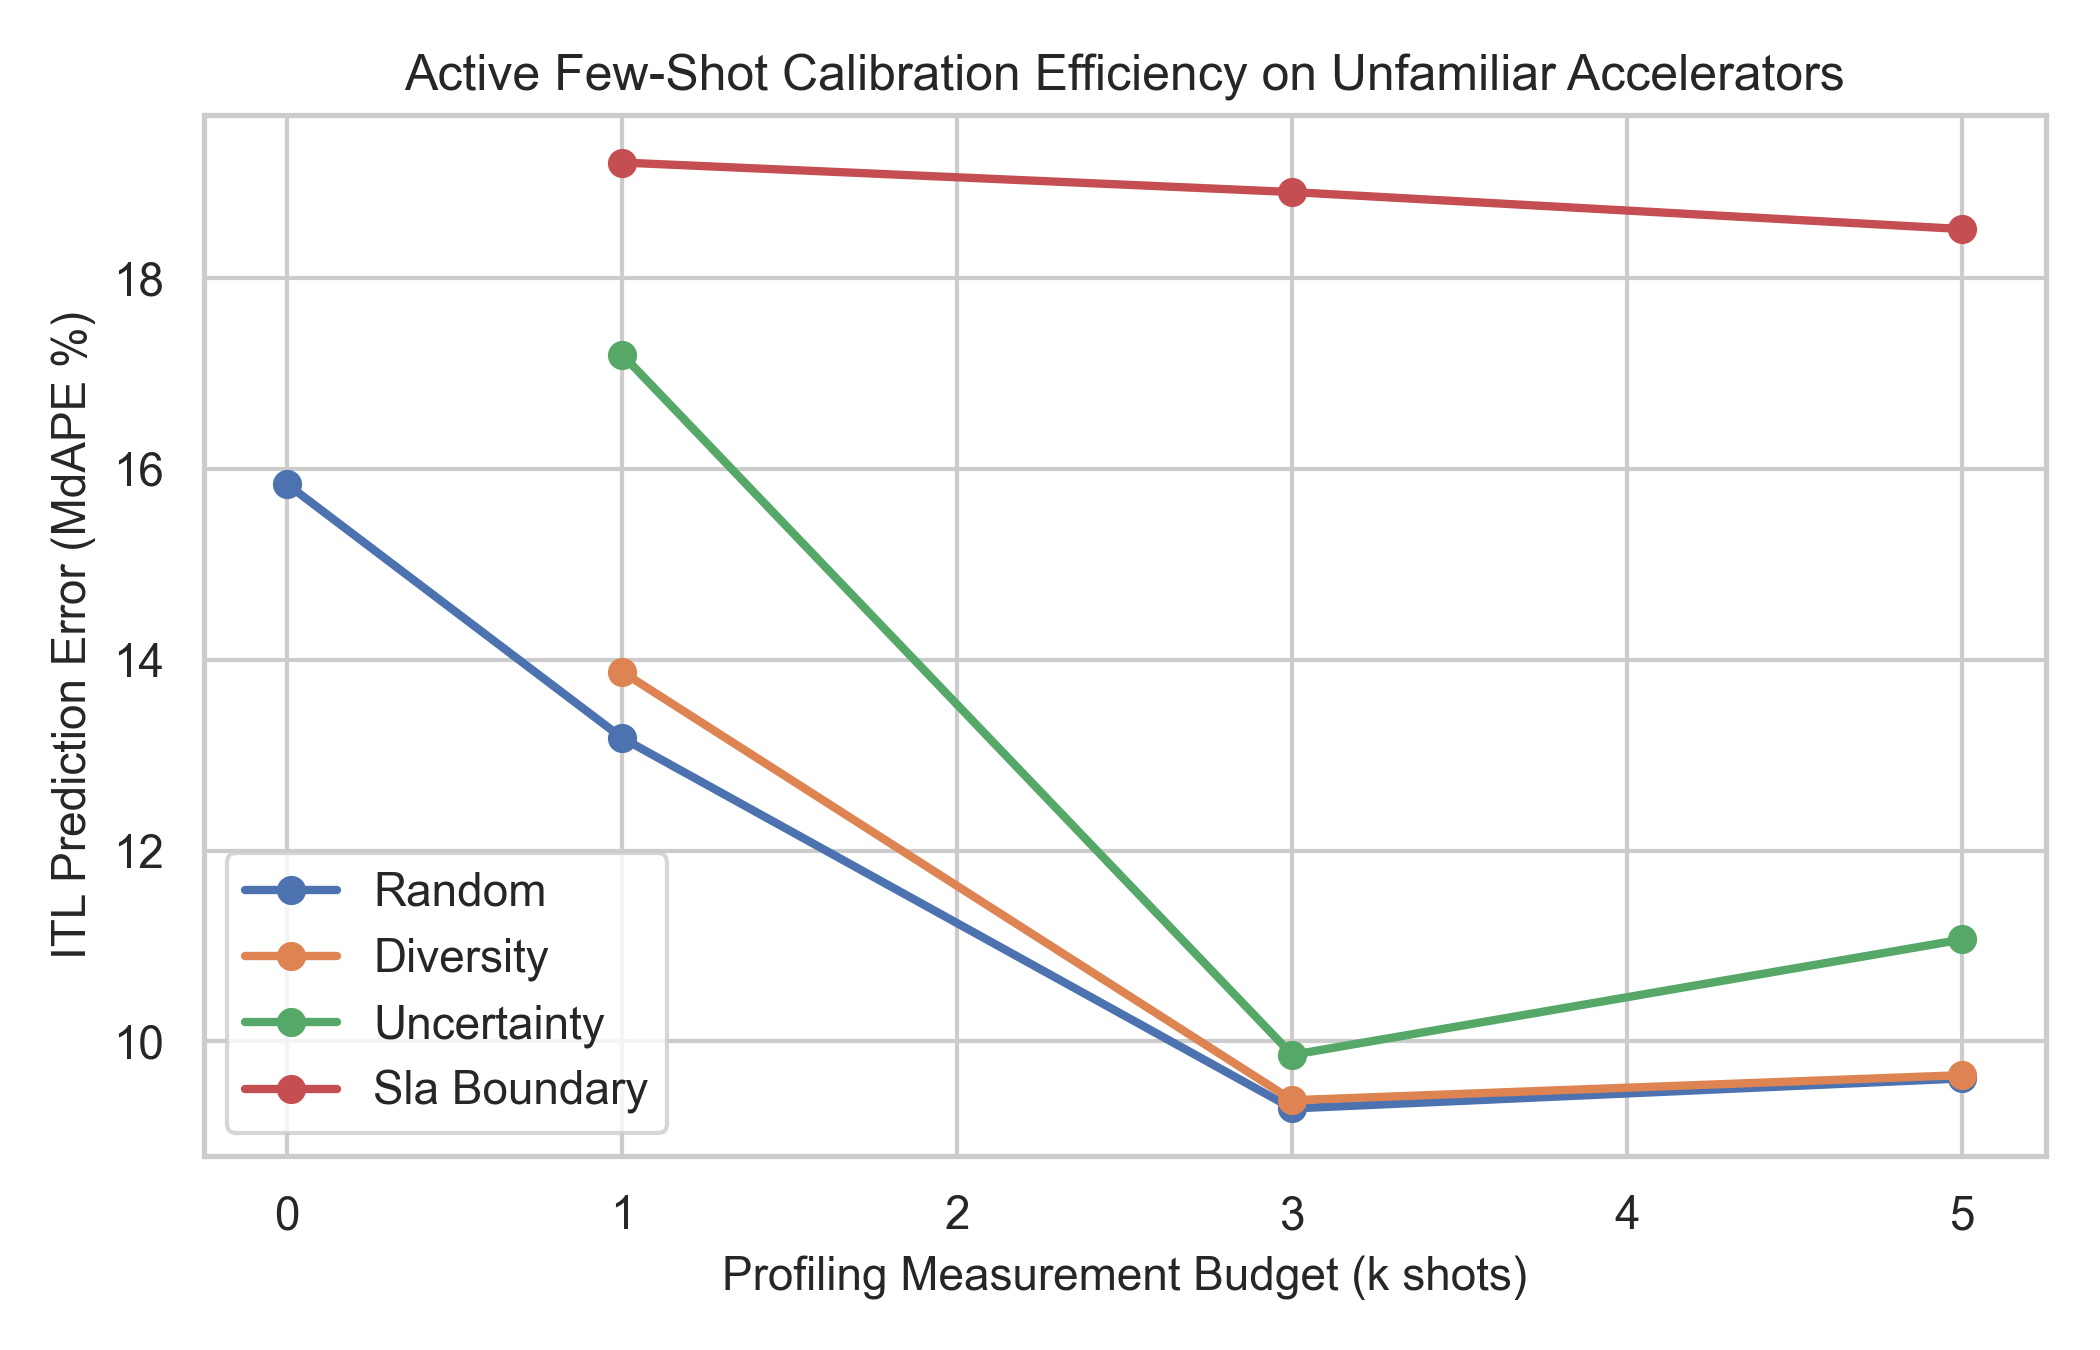
\includegraphics[width=0.84\linewidth]{figures/fig2_few_shot_adaptation_curves.png}}
\caption{Latency error across profiling strategies and
budgets.}
\end{figure}

\section{Discussion and Systems
Implications}\label{discussion-and-systems-implications}

\subsection{Operational Energy vs.~Instantaneous
Power}\label{operational-energy-vs.-instantaneous-power}

A common misconception in AI infrastructure is treating instantaneous
GPU power draw (Watts) as synonymous with energy consumption (Joules).
In autoregressive inference, total energy per request is the time
integral of power: $E = \int P(t)\,dt$. A low-TDP accelerator (e.g., Tesla T4
at 70 W) operating at high latency may consume significantly more total
energy than an advanced accelerator (e.g., L40S at 350 W) that finishes
the inference burst in a fraction of the time. The reported benchmark
compares mean GPU power. Energy per generated token requires separate
accounting for runtime and completed work.

\section{Threats to Validity and
Limitations}\label{threats-to-validity-and-limitations}

This evaluation supports an offline comparison on the available
benchmark. It uses one split seed and eight NVIDIA devices on one
serving stack. Candidate availability follows the benchmark and may
differ from a production cluster. Coverage under a new GPU family,
request tail latency, performance under different runtimes, and the
effect of active profiling on final hardware decisions remain open. A
trained attention ablation would help establish what the architecture
adds. Power in watts is a rate. Joules per generated token and profiling
energy require measured duration, work completed, and appropriate
accounting for each experiment.

\section{Conclusion}\label{conclusion}

The interval adjustment improved empirical coverage on the benchmark and
reduced observed violations in offline replay at higher selected power.
Three randomly selected probes reduced latency error on the shared
evaluation set from 15.84\% to 9.30\%. The SLA boundary heuristic did
not beat random selection at any evaluated budget. These results
motivate studying profiling and selection as separate decisions and
testing them together on additional hardware.

\section*{CRediT Authorship Contribution
Statement}\label{credit-authorship-contribution-statement}

\textbf{Jason Pandian:} Conceptualization, Methodology, Software,
Validation, Formal analysis, Investigation, Data Curation, Writing -
Original Draft, Writing - Review \& Editing, Visualization, Supervision,
Project administration, Resources.

\begin{center}\rule{0.5\linewidth}{0.5pt}\end{center}

\section*{Declaration of Competing
Interest}\label{declaration-of-competing-interest}

The author declares that he has no known competing financial interests
or personal relationships that could have appeared to influence the work
reported in this paper.

\begin{center}\rule{0.5\linewidth}{0.5pt}\end{center}

\section*{Data and code availability}\label{data-and-code-availability}

The benchmark data accompany
\href{https://github.com/maufadel/wattgpu}{WattGPU}. The revised
implementation, experiment runner, and generated tables accompany this
draft.

\section*{Author Biographies}\label{author-biographies}

\textbf{Jason Pandian} received his B.E. degree in Computer Science and
Engineering and M.E. degree in Information Technology. He is currently
pursuing his Ph.D.~degree in the Department of Information Technology at
Nehru Institute of Technology, Coimbatore, Tamil Nadu, India. His
research interests include distributed AI infrastructure, GPU computing,
sustainable cloud data centers, deep learning performance modeling, and
uncertainty quantification.

\begin{center}\rule{0.5\linewidth}{0.5pt}\end{center}
\begin{thebibliography}{99}
\bibitem{r1} Castaño, J., Bustillo, J., Franch, X., and Martínez-Fernández, S.
(2026). Data-driven multi-objective optimization of ML inference
hardware configurations for energy, performance and cost.
\emph{Sustainable Computing: Informatics and Systems}, 50, 101347.
\href{https://doi.org/10.1016/j.suscom.2026.101347}{DOI}.

\bibitem{r2} Aguirre-Usandizaga, J., Torre-Bastida, A. I., Linares de la Puerta, M.,
and Almeida, A. (2026). A forecasting-based perception layer for
energy-aware resource management in LLM serving deployed on
high-performance computing clusters. \emph{Sustainable Computing:
Informatics and Systems}, 50, 101333.
\href{https://doi.org/10.1016/j.suscom.2026.101333}{DOI}.

\bibitem{r3} Fadel Argerich, M., Fürst, J., and Patiño-Martínez, M. (2026). WattGPU:
Predicting inference power and latency on unseen GPUs and LLMs.
\href{https://arxiv.org/abs/2607.02391}{arXiv:2607.02391}.

\bibitem{r4} Imai, S., Nakazawa, R., Amaral, M., Choochotkaew, S., and Chiba, T.
(2024). Predicting LLM Inference Latency: A Roofline-Driven ML Method.
NeurIPS workshop paper.
\href{https://research.ibm.com/publications/predicting-llm-inference-latency-a-roofline-driven-ml-method}{IBM
Research}.

\bibitem{r5} Lee, S., Phanishayee, A., and Mahajan, D. (2025). Forecasting GPU
Performance for Deep Learning Training and Inference. ASPLOS 2025.
\href{https://arxiv.org/abs/2407.13853}{arXiv:2407.13853}.

\bibitem{r6} Tibshirani, R. J., Barber, R. F., Candès, E., and Ramdas, A. (2019).
Conformal prediction under covariate shift. \emph{Advances in Neural
Information Processing Systems}, 32.
\href{https://proceedings.neurips.cc/paper/2019/hash/8fb21ee7a2207526da55a679f0332de2-Abstract.html}{Proceedings}.

\bibitem{r7} Williams, S., Waterman, A., and Patterson, D. (2009). Roofline: An
insightful visual performance model for multicore architectures.
\emph{Communications of the ACM}, 52(4), 65--76.
\href{https://doi.org/10.1145/1498765.1498785}{DOI}.
\end{thebibliography}
\end{document}